\documentclass[12pt,pdftex,a4paper]{article}

%------------------------------------------------------------Packages------------------------------------------------------------
\usepackage[ngerman]{babel}
\usepackage[utf8]{inputenc}
\usepackage[T1]{fontenc}
\usepackage[left=2cm, right=2cm, top=1.50cm, bottom=1.5cm]{geometry}
\usepackage{setspace}
\usepackage{tabularx}
\usepackage{amsmath}
\usepackage{tikz}
\usepackage{tikz-cd}
\usepackage{amssymb}
\usepackage{graphicx}
\usepackage{amsmath}
\onehalfspacing
\usepackage{listings}
\usepackage{color}
\usepackage{hyperref}
\usepackage{fancyhdr}
%------------------------------------------------------------Packages------------------------------------------------------------

%------------------------------------------------------------Title---------------------------------------------------------------
\title{\vspace{-1cm} Software Engineering \\ Exercise 1}
\author{\textbf{Jonas Allali}\\ 2965826\\st116462@stud.uni-stuttgart.de \and \textbf{Timo Hüttner}\\ 3220544\\ st148236@stud.uni-stuttgart.de \and \textbf{Heinrich Pauli}\\ 3245875\\st150482@stud.uni-stuttgart.de \and \textbf{Jena Satkunarajan}\\2965839\\st116472@stud.uni-stuttgart.de}
\date{}
\makeatletter
\let\gruppe\@author
\let\titel\@title
\makeatother
\pagestyle{fancy}
\lhead{SE, Exercise 1}
\rhead{2965826, 3220544, 3245875, 2965839\\ Jonas Allali, Timo Hüttner, Heinrich Pauli, Jena Satkunarajan}
\headheight = 15pt
\topmargin = -35pt
%------------------------------------------------------------Title---------------------------------------------------------------


\begin{document}

%------------------------------------------------------------Set Up Title Page---------------------------------------------------
\setlength{\parindent}{0pt}
\maketitle
\thispagestyle{fancy}
\newpage
%------------------------------------------------------------Set Up Title Page---------------------------------------------------


%------------------------------------------------------------Content-------------------------------------------------------------
\section*{Aufgabe 1: Kritischer Pfad)}

\subsection*{a)}

\begin{figure}[htbp]
\centering
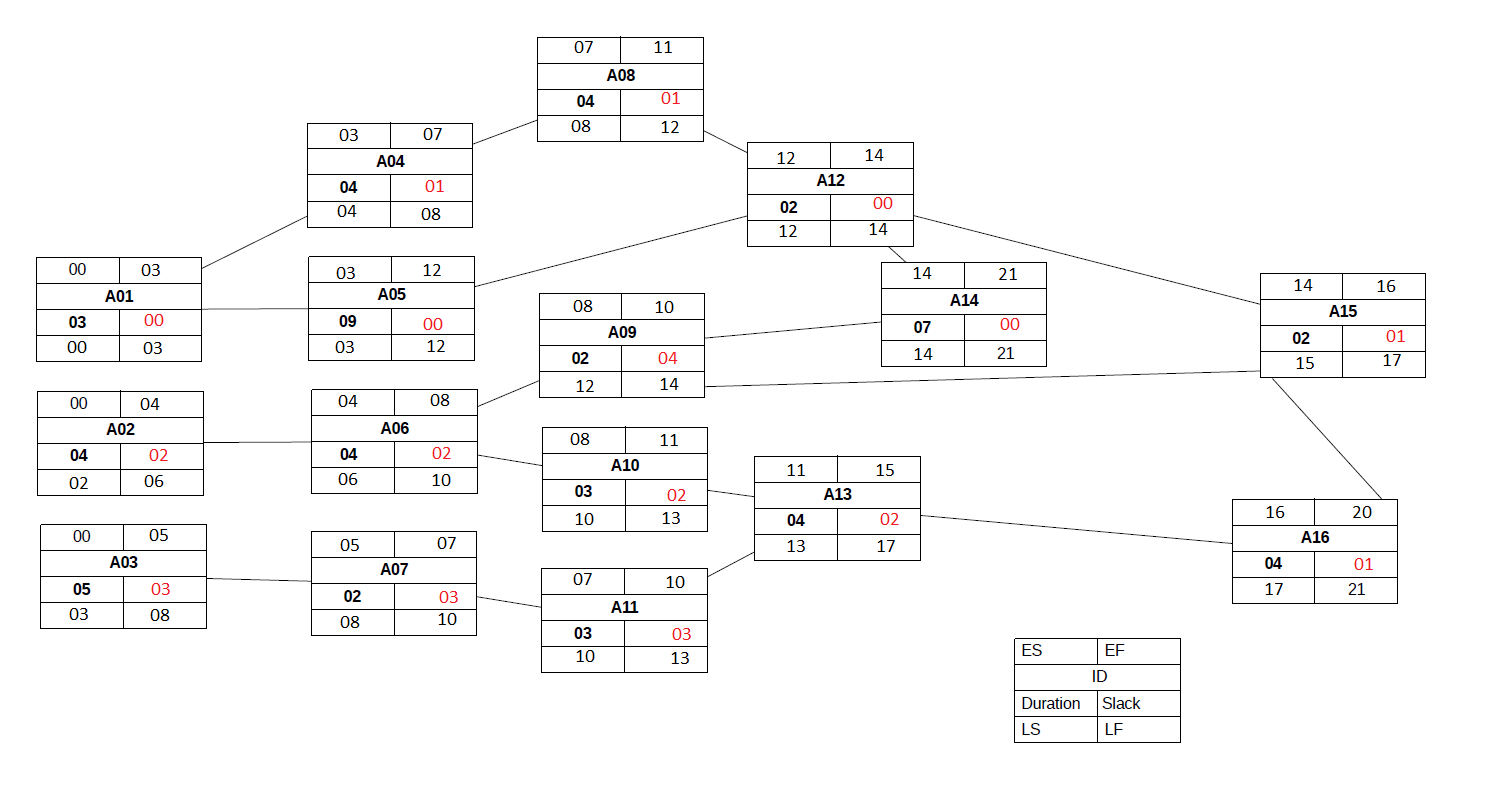
\includegraphics[width=1\textwidth]{1a.png}
\end{figure}

\section*{\underline{Aufgabe 2: Ressourcenmanagament}}
\subsection*{a)}
Es liegt eine kapazitätsgetreue Einsatzplanung vor, da das zur Verfügung stehende Personal dem Auftragnehmer, in diesem Fall die Firma, bekannt beziehungsweise vorgegeben ist, während der frühstmögliche/optimale Fertigstellungstermin des Softwareprojekts anhand der Vorgaben ermittelt werden muss.

\newpage
\subsection*{b)}
\begin{figure}[htbp]
\centering
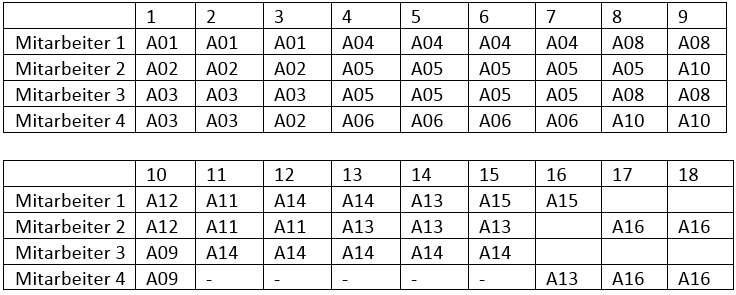
\includegraphics[width=1\textwidth]{2b.png}
\end{figure}

Es benötigt mindestens 17 Arbeitstage, um sämtliche Arbeitspakete unter Einhaltung der firmeninternen Richtlinen abzuarbeiten.

\subsection*{c)}

Insgesamt müsste ein Mitarbeiter 62 Arbeitstage aufbringen, um das Projekt abzuschließen. Also müssten mindestens 7 Mitarbeiter eingestellt werden.

\subsection*{d)}

Aufgrund der Abhängigkeiten der Arbeitspakete wäre das nicht möglich, als Beispiel sei der kritische Pfad bestehend aus A01, A05, A12 und A14 genannt, welcher mit nur zwei Mitarbeitern bereits 10,5 Personentage brauchen würde.

\newpage
\section*{Aufgabe 3: Gantt-Diagramm, Termin-Drift-Diagramm}

\subsection*{a)}
\begin{figure}[htbp]
\centering
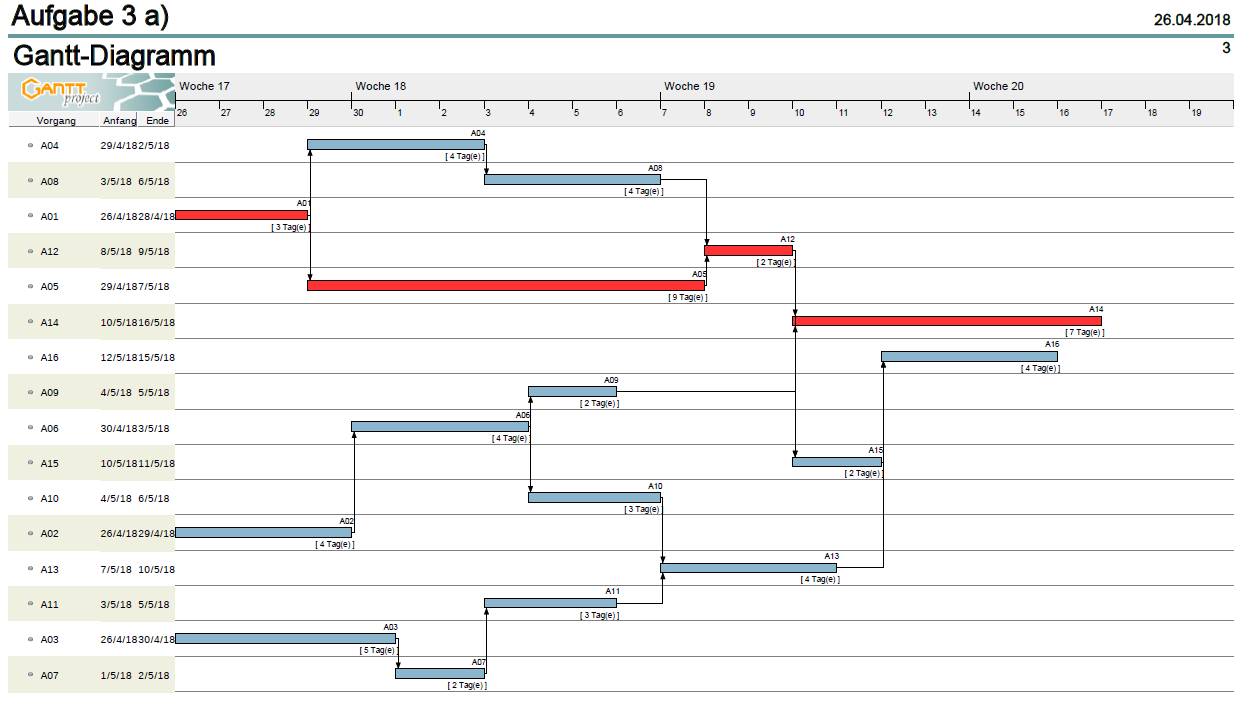
\includegraphics[width=1\textwidth]{3a.png}
\end{figure}

\subsection*{b)}

\begin{itemize}

\item \textbf{\underline{Wurde das Projekt rechtzeitig abgeschlossen?}}\\
Das Projekt wurde rechtzeitig abgeschlossen, da der letzte Meilenstein rechtzeitig abgeschlossen wurde.

\item \textbf{\underline{Welche Meilensteine wurden pünktlich/früher/später erreicht?}}\\
Meilenstein E und S wurden früher abgeschlossen als geplant. Meilenstein I wurde später abgeschlossen als geplant. Meilenstein T und A wurden rechtzeitig abgeschlossen.

\item \textbf{\underline{Wie oft wurden Meilensteine jeweils verlegt?}}\\
Meilenstein S wurde 2-mal verlegt, Meilenstein E einmal und Meilenstein I einmal. T und A wurden nicht verlegt.

\item \textbf{\underline{Welche Phasen waren länger/kürzer als geplant?}}\\
Die Phase der Spezifikation war kürzer als geplant.  Auch die Phase des Entwurfs war kürzer als geplant. Die Phase der Implementierung war viel länger als geplant.\\
Die Phase des Tests war viel kürzer als geplant.

\newpage
\item \textbf{\underline{Muss das Schätzverfahren verbessert werden?}}\\
Es ist ganz normal für Projekte, dass sie ihre Meilensteine nicht perfekt einschätzbar sind. Besonders nicht am Anfang des Projekts. Jedoch sollte stetig versucht werden seine Schätzungen zu verbessern. Jedes Schätzverfahren kann immer verbessert werden. Besonders bei der Programmierphase hätte man eine bessere Schätzung sehr benötigt.

\item \textbf{\underline{Vermutungen:}}\\
Spezifikation und Entwurf liefen schneller als geplant, da der Kunde dieses Mal womöglich ganz genau wusste, was entwickelt werden sollte, wodurch etwas Zeit in diesen Phasen gespart werden konnte.\\

Der Programmieraufwand wurde vielleicht unterschätzt, da unsere Kollegen vielleicht eine neue Programmiersprache, mit welcher sie nicht zurechtkamen, verwendeten. Vielleicht gab es Probleme bei den Absprachen untereinander. Es könnte auch das ganze Team plötzlich erkrankt sein. Man sieht klar im Diagramm, dass beim Programmieren etwas sehr schief lief.\\

Die Tests werden nicht gut funktioniert haben. Wahrscheinlich wird das Programm einige Fehler haben, da die Testphase viel zu kurz kam. Es wird wahrscheinlich keine hohe Testabdeckung geben. Um den Meilenstein noch rechtzeitig zu erreichen, wurden die Tests wohl als nicht wichtig betrachtet.

\end{itemize}

%------------------------------------------------------------Content-------------------------------------------------------------



\end{document}